
%% bare_conf.tex
%% V1.4
%% 2012/12/27
%% by Michael Shell
%% See:
%% http://www.michaelshell.org/
%% for current contact information.
%%
%% This is a skeleton file demonstrating the use of IEEEtran.cls
%% (requires IEEEtran.cls version 1.8 or later) with an IEEE conference paper.
%%
%% Support sites:
%% http://www.michaelshell.org/tex/ieeetran/
%% http://www.ctan.org/tex-archive/macros/latex/contrib/IEEEtran/
%% and
%% http://www.ieee.org/

%%*************************************************************************
%% Legal Notice:
%% This code is offered as-is without any warranty either expressed or
%% implied; without even the implied warranty of MERCHANTABILITY or
%% FITNESS FOR A PARTICULAR PURPOSE!
%% User assumes all risk.
%% In no event shall IEEE or any contributor to this code be liable for
%% any damages or losses, including, but not limited to, incidental,
%% consequential, or any other damages, resulting from the use or misuse
%% of any information contained here.
%%
%% All comments are the opinions of their respective authors and are not
%% necessarily endorsed by the IEEE.
%%
%% This work is distributed under the LaTeX Project Public License (LPPL)
%% ( http://www.latex-project.org/ ) version 1.3, and may be freely used,
%% distributed and modified. A copy of the LPPL, version 1.3, is included
%% in the base LaTeX documentation of all distributions of LaTeX released
%% 2003/12/01 or later.
%% Retain all contribution notices and credits.
%% ** Modified files should be clearly indicated as such, including  **
%% ** renaming them and changing author support contact information. **
%%
%% File list of work: IEEEtran.cls, IEEEtran_HOWTO.pdf, bare_adv.tex,
%%                    bare_conf.tex, bare_jrnl.tex, bare_jrnl_compsoc.tex,
%%                    bare_jrnl_transmag.tex
%%*************************************************************************

% *** Authors should verify (and, if needed, correct) their LaTeX system  ***
% *** with the testflow diagnostic prior to trusting their LaTeX platform ***
% *** with production work. IEEE's font choices can trigger bugs that do  ***
% *** not appear when using other class files.                            ***
% The testflow support page is at:
% http://www.michaelshell.org/tex/testflow/



% Note that the a4paper option is mainly intended so that authors in
% countries using A4 can easily print to A4 and see how their papers will
% look in print - the typesetting of the document will not typically be
% affected with changes in paper size (but the bottom and side margins will).
% Use the testflow package mentioned above to verify correct handling of
% both paper sizes by the user's LaTeX system.
%
% Also note that the "draftcls" or "draftclsnofoot", not "draft", option
% should be used if it is desired that the figures are to be displayed in
% draft mode.
%
\documentclass[conference]{IEEEtran}
\usepackage{amsmath}
\usepackage{mathtools}
\usepackage{listings}

\usepackage{color}
% Add the compsoc option for Computer Society conferences.
%
% If IEEEtran.cls has not been installed into the LaTeX system files,
% manually specify the path to it like:
% \documentclass[conference]{../sty/IEEEtran}





% Some very useful LaTeX packages include:
% (uncomment the ones you want to load)


% *** MISC UTILITY PACKAGES ***
%
%\usepackage{ifpdf}
% Heiko Oberdiek's ifpdf.sty is very useful if you need conditional
% compilation based on whether the output is pdf or dvi.
% usage:
% \ifpdf
%   % pdf code
% \else
%   % dvi code
% \fi
% The latest version of ifpdf.sty can be obtained from:
% http://www.ctan.org/tex-archive/macros/latex/contrib/oberdiek/
% Also, note that IEEEtran.cls V1.7 and later provides a builtin
% \ifCLASSINFOpdf conditional that works the same way.
% When switching from latex to pdflatex and vice-versa, the compiler may
% have to be run twice to clear warning/error messages.






% *** CITATION PACKAGES ***
%
%\usepackage{cite}
% cite.sty was written by Donald Arseneau
% V1.6 and later of IEEEtran pre-defines the format of the cite.sty package
% \cite{} output to follow that of IEEE. Loading the cite package will
% result in citation numbers being automatically sorted and properly
% "compressed/ranged". e.g., [1], [9], [2], [7], [5], [6] without using
% cite.sty will become [1], [2], [5]--[7], [9] using cite.sty. cite.sty's
% \cite will automatically add leading space, if needed. Use cite.sty's
% noadjust option (cite.sty V3.8 and later) if you want to turn this off
% such as if a citation ever needs to be enclosed in parenthesis.
% cite.sty is already installed on most LaTeX systems. Be sure and use
% version 4.0 (2003-05-27) and later if using hyperref.sty. cite.sty does
% not currently provide for hyperlinked citations.
% The latest version can be obtained at:
% http://www.ctan.org/tex-archive/macros/latex/contrib/cite/
% The documentation is contained in the cite.sty file itself.






% *** GRAPHICS RELATED PACKAGES ***
%
\ifCLASSINFOpdf
\usepackage[pdftex]{graphicx}
  % declare the path(s) where your graphic files are
  % \graphicspath{{../pdf/}{../jpeg/}}
  % and their extensions so you won't have to specify these with
  % every instance of \includegraphics
  % \DeclareGraphicsExtensions{.pdf,.jpeg,.png}
\else
  % or other class option (dvipsone, dvipdf, if not using dvips). graphicx
  % will default to the driver specified in the system graphics.cfg if no
  % driver is specified.
  % \usepackage[dvips]{graphicx}
  % declare the path(s) where your graphic files are
  % \graphicspath{{../eps/}}
  % and their extensions so you won't have to specify these with
  % every instance of \includegraphics
  % \DeclareGraphicsExtensions{.eps}
\fi
% graphicx was written by David Carlisle and Sebastian Rahtz. It is
% required if you want graphics, photos, etc. graphicx.sty is already
% installed on most LaTeX systems. The latest version and documentation
% can be obtained at:
% http://www.ctan.org/tex-archive/macros/latex/required/graphics/
% Another good source of documentation is "Using Imported Graphics in
% LaTeX2e" by Keith Reckdahl which can be found at:
% http://www.ctan.org/tex-archive/info/epslatex/
%
% latex, and pdflatex in dvi mode, support graphics in encapsulated
% postscript (.eps) format. pdflatex in pdf mode supports graphics
% in .pdf, .jpeg, .png and .mps (metapost) formats. Users should ensure
% that all non-photo figures use a vector format (.eps, .pdf, .mps) and
% not a bitmapped formats (.jpeg, .png). IEEE frowns on bitmapped formats
% which can result in "jaggedy"/blurry rendering of lines and letters as
% well as large increases in file sizes.
%
% You can find documentation about the pdfTeX application at:
% http://www.tug.org/applications/pdftex





% *** MATH PACKAGES ***
%
%\usepackage[cmex10]{amsmath}
% A popular package from the American Mathematical Society that provides
% many useful and powerful commands for dealing with mathematics. If using
% it, be sure to load this package with the cmex10 option to ensure that
% only type 1 fonts will utilized at all point sizes. Without this option,
% it is possible that some math symbols, particularly those within
% footnotes, will be rendered in bitmap form which will result in a
% document that can not be IEEE Xplore compliant!
%
% Also, note that the amsmath package sets \interdisplaylinepenalty to 10000
% thus preventing page breaks from occurring within multiline equations. Use:
%\interdisplaylinepenalty=2500
% after loading amsmath to restore such page breaks as IEEEtran.cls normally
% does. amsmath.sty is already installed on most LaTeX systems. The latest
% version and documentation can be obtained at:
% http://www.ctan.org/tex-archive/macros/latex/required/amslatex/math/





% *** SPECIALIZED LIST PACKAGES ***
%
\usepackage{algorithm}
\usepackage{algorithmic}
% algorithmic.sty was written by Peter Williams and Rogerio Brito.
% This package provides an algorithmic environment fo describing algorithms.
% You can use the algorithmic environment in-text or within a figure
% environment to provide for a floating algorithm. Do NOT use the algorithm
% floating environment provided by algorithm.sty (by the same authors) or
% algorithm2e.sty (by Christophe Fiorio) as IEEE does not use dedicated
% algorithm float types and packages that provide these will not provide
% correct IEEE style captions. The latest version and documentation of
% algorithmic.sty can be obtained at:
% http://www.ctan.org/tex-archive/macros/latex/contrib/algorithms/
% There is also a support site at:
% http://algorithms.berlios.de/index.html
% Also of interest may be the (relatively newer and more customizable)
% algorithmicx.sty package by Szasz Janos:
% http://www.ctan.org/tex-archive/macros/latex/contrib/algorithmicx/




% *** ALIGNMENT PACKAGES ***
%
%\usepackage{array}
% Frank Mittelbach's and David Carlisle's array.sty patches and improves
% the standard LaTeX2e array and tabular environments to provide better
% appearance and additional user controls. As the default LaTeX2e table
% generation code is lacking to the point of almost being broken with
% respect to the quality of the end results, all users are strongly
% advised to use an enhanced (at the very least that provided by array.sty)
% set of table tools. array.sty is already installed on most systems. The
% latest version and documentation can be obtained at:
% http://www.ctan.org/tex-archive/macros/latex/required/tools/


% IEEEtran contains the IEEEeqnarray family of commands that can be used to
% generate multiline equations as well as matrices, tables, etc., of high
% quality.




% *** SUBFIGURE PACKAGES ***
%\ifCLASSOPTIONcompsoc
%  \usepackage[caption=false,font=normalsize,labelfont=sf,textfont=sf]{subfig}
%\else
%  \usepackage[caption=false,font=footnotesize]{subfig}
%\fi
% subfig.sty, written by Steven Douglas Cochran, is the modern replacement
% for subfigure.sty, the latter of which is no longer maintained and is
% incompatible with some LaTeX packages including fixltx2e. However,
% subfig.sty requires and automatically loads Axel Sommerfeldt's caption.sty
% which will override IEEEtran.cls' handling of captions and this will result
% in non-IEEE style figure/table captions. To prevent this problem, be sure
% and invoke subfig.sty's "caption=false" package option (available since
% subfig.sty version 1.3, 2005/06/28) as this is will preserve IEEEtran.cls
% handling of captions.
% Note that the Computer Society format requires a larger sans serif font
% than the serif footnote size font used in traditional IEEE formatting
% and thus the need to invoke different subfig.sty package options depending
% on whether compsoc mode has been enabled.
%
% The latest version and documentation of subfig.sty can be obtained at:
% http://www.ctan.org/tex-archive/macros/latex/contrib/subfig/




% *** FLOAT PACKAGES ***
%
%\usepackage{fixltx2e}
% fixltx2e, the successor to the earlier fix2col.sty, was written by
% Frank Mittelbach and David Carlisle. This package corrects a few problems
% in the LaTeX2e kernel, the most notable of which is that in current
% LaTeX2e releases, the ordering of single and double column floats is not
% guaranteed to be preserved. Thus, an unpatched LaTeX2e can allow a
% single column figure to be placed prior to an earlier double column
% figure. The latest version and documentation can be found at:
% http://www.ctan.org/tex-archive/macros/latex/base/


%\usepackage{stfloats}
% stfloats.sty was written by Sigitas Tolusis. This package gives LaTeX2e
% the ability to do double column floats at the bottom of the page as well
% as the top. (e.g., "\begin{figure*}[!b]" is not normally possible in
% LaTeX2e). It also provides a command:
%\fnbelowfloat
% to enable the placement of footnotes below bottom floats (the standard
% LaTeX2e kernel puts them above bottom floats). This is an invasive package
% which rewrites many portions of the LaTeX2e float routines. It may not work
% with other packages that modify the LaTeX2e float routines. The latest
% version and documentation can be obtained at:
% http://www.ctan.org/tex-archive/macros/latex/contrib/sttools/
% Do not use the stfloats baselinefloat ability as IEEE does not allow
% \baselineskip to stretch. Authors submitting work to the IEEE should note
% that IEEE rarely uses double column equations and that authors should try
% to avoid such use. Do not be tempted to use the cuted.sty or midfloat.sty
% packages (also by Sigitas Tolusis) as IEEE does not format its papers in
% such ways.
% Do not attempt to use stfloats with fixltx2e as they are incompatible.
% Instead, use Morten Hogholm'a dblfloatfix which combines the features
% of both fixltx2e and stfloats:
%
% \usepackage{dblfloatfix}
% The latest version can be found at:
% http://www.ctan.org/tex-archive/macros/latex/contrib/dblfloatfix/




% *** PDF, URL AND HYPERLINK PACKAGES ***
%
%\usepackage{url}
% url.sty was written by Donald Arseneau. It provides better support for
% handling and breaking URLs. url.sty is already installed on most LaTeX
% systems. The latest version and documentation can be obtained at:
% http://www.ctan.org/tex-archive/macros/latex/contrib/url/
% Basically, \url{my_url_here}.




% *** Do not adjust lengths that control margins, column widths, etc. ***
% *** Do not use packages that alter fonts (such as pslatex).         ***
% There should be no need to do such things with IEEEtran.cls V1.6 and later.
% (Unless specifically asked to do so by the journal or conference you plan
% to submit to, of course. )

% correct bad hyphenation here
\hyphenation{op-tical net-works semi-conduc-tor}

\begin{document}
%
% paper title
% can use linebreaks \\ within to get better formatting as desired
% Do not put math or special symbols in the title.
\title{Cross Block Chaining Security Analysis}

% author names and affiliations
% use a multiple column layout for up to three different
% affiliations
\author{
\IEEEauthorblockN{Minal Tolpadi}
\IEEEauthorblockA{College of Computing\\
Georgia Institute of Technology\\
Atlanta, Georgia 30332--0250\\
Email: mtolpadi3@gatech.edu}
\and
\IEEEauthorblockN{Vojtech Miksu}
\IEEEauthorblockA{College of Computing\\
Georgia Institute of Technology\\
Atlanta, Georgia 30332--0250\\
Email: miksu@gatech.edu}
\and
\IEEEauthorblockN{Nils Gustav Davidsson}
\IEEEauthorblockA{College of Computing\\
Georgia Institute of Technology\\
Atlanta, Georgia 30332--0250\\
Email: gustav@gatech.edu}
}

% conference papers do not typically use \thanks and this command
% is locked out in conference mode. If really needed, such as for
% the acknowledgment of grants, issue a \IEEEoverridecommandlockouts
% after \documentclass

% for over three affiliations, or if they all won't fit within the width
% of the page, use this alternative format:
%
%\author{\IEEEauthorblockN{Michael Shell\IEEEauthorrefmark{1},
%Homer Simpson\IEEEauthorrefmark{2},
%James Kirk\IEEEauthorrefmark{3},
%Montgomery Scott\IEEEauthorrefmark{3} and
%Eldon Tyrell\IEEEauthorrefmark{4}}
%\IEEEauthorblockA{\IEEEauthorrefmark{1}School of Electrical and Computer Engineering\\
%Georgia Institute of Technology,
%Atlanta, Georgia 30332--0250\\ Email: see http://www.michaelshell.org/contact.html}
%\IEEEauthorblockA{\IEEEauthorrefmark{2}Twentieth Century Fox, Springfield, USA\\
%Email: homer@thesimpsons.com}
%\IEEEauthorblockA{\IEEEauthorrefmark{3}Starfleet Academy, San Francisco, California 96678-2391\\
%Telephone: (800) 555--1212, Fax: (888) 555--1212}
%\IEEEauthorblockA{\IEEEauthorrefmark{4}Tyrell Inc., 123 Replicant Street, Los Angeles, California 90210--4321}}




% use for special paper notices
%\IEEEspecialpapernotice{(Invited Paper)}




% make the title area
\maketitle

% As a general rule, do not put math, special symbols or citations
% in the abstract
\begin{abstract}
Cross Block Chaining (XBC) is a mode of operation for a block cipher. It resembles one of the most used modes - Cipher Block Chaining (CBC). However, it operates using two IVs instead of one, which introduces new capabilities but also raises security concerns. Our work focuses on a detailed security analysis of the Cross Block Chaining mode. We show a proof for XBC being IND-CPA secure and IND-CCA insecure. We also discuss importance of initialization vector selection and its consequences on the scheme security.
\end{abstract}

% As a general rule, do not put math, special symbols or citations
% in the abstract
\begin{keywords}
cross block chaining; XBC; IND-CPA; IND-CCA; security analysis
\end{keywords}

% no keywords
% For peer review papers, you can put extra information on the cover
% page as needed:
% \ifCLASSOPTIONpeerreview
% \begin{center} \bfseries EDICS Category: 3-BBND \end{center}
% \fi
%
% For peerreview papers, this IEEEtran command inserts a page break and
% creates the second title. It will be ignored for other modes.
\IEEEpeerreviewmaketitle

\section{Introduction}
% no \IEEEPARstart

Since a block cipher by itself is suitable only for encryption or decryption of one length-fixed block of bits, there is a need to introduce an algorithm, a mode of operation, that uses the block cipher as a underlying building block and enables us to encrypt or decrypt a message of variable length. There are many modes in a widespread use: Electronic Codebook (EBC), Cipher Block Chaining (CBC), Cipher Feedback (CFB), Output Feedback (OFB) or Counter (CTR).

In May 2014, Andre Watson submitted a proposal for a new block cipher mode of operation called Cross Block Chaining (XBC). This proposal was published by National Institute of Standards and Technology (NIST) under the proposed modes section. However, no formal proof considering security has been made.

Section II talks about the fundamentals and design of the XBC mode and its two main variants. Section III describes security analysis and provides various attacks that can be used against the XBC scheme. Section IV shows an intuition for the proof of IND-CPA security of XBC mode. The last part is conclusion.

% An example of a floating figure using the graphicx package.
% Note that \label must occur AFTER (or within) \caption.
% For figures, \caption should occur after the \includegraphics.
% Note that IEEEtran v1.7 and later has special internal code that
% is designed to preserve the operation of \label within \caption
% even when the captionsoff option is in effect. However, because
% of issues like this, it may be the safest practice to put all your
% \label just after \caption rather than within \caption{}.
%
% Reminder: the "draftcls" or "draftclsnofoot", not "draft", class
% option should be used if it is desired that the figures are to be
% displayed while in draft mode.
%
%\begin{figure}[!t]
%\centering
%\includegraphics[width=2.5in]{myfigure}
% where an .eps filename suffix will be assumed under latex,
% and a .pdf suffix will be assumed for pdflatex; or what has been declared
% via \DeclareGraphicsExtensions.
%\caption{Simulation Results.}
%\label{fig_sim}
%\end{figure}

% Note that IEEE typically puts floats only at the top, even when this
% results in a large percentage of a column being occupied by floats.


% An example of a double column floating figure using two subfigures.
% (The subfig.sty package must be loaded for this to work.)
% The subfigure \label commands are set within each subfloat command,
% and the \label for the overall figure must come after \caption.
% \hfil is used as a separator to get equal spacing.
% Watch out that the combined width of all the subfigures on a
% line do not exceed the text width or a line break will occur.
%
%\begin{figure*}[!t]
%\centering
%\subfloat[Case I]{\includegraphics[width=2.5in]{box}%
%\label{fig_first_case}}
%\hfil
%\subfloat[Case II]{\includegraphics[width=2.5in]{box}%
%\label{fig_second_case}}
%\caption{Simulation results.}
%\label{fig_sim}
%\end{figure*}
%
% Note that often IEEE papers with subfigures do not employ subfigure
% captions (using the optional argument to \subfloat[]), but instead will
% reference/describe all of them (a), (b), etc., within the main caption.


% An example of a floating table. Note that, for IEEE style tables, the
% \caption command should come BEFORE the table. Table text will default to
% \footnotesize as IEEE normally uses this smaller font for tables.
% The \label must come after \caption as always.
%
%\begin{table}[!t]
%% increase table row spacing, adjust to taste
%\renewcommand{\arraystretch}{1.3}
% if using array.sty, it might be a good idea to tweak the value of
% \extrarowheight as needed to properly center the text within the cells
%\caption{An Example of a Table}
%\label{table_example}
%\centering
%% Some packages, such as MDW tools, offer better commands for making tables
%% than the plain LaTeX2e tabular which is used here.
%\begin{tabular}{|c||c|}
%\hline
%One & Two\\
%\hline
%Three & Four\\
%\hline
%\end{tabular}
%\end{table}


% Note that IEEE does not put floats in the very first column - or typically
% anywhere on the first page for that matter. Also, in-text middle ("here")
% positioning is not used. Most IEEE journals/conferences use top floats
% exclusively. Note that, LaTeX2e, unlike IEEE journals/conferences, places
% footnotes above bottom floats. This can be corrected via the \fnbelowfloat
% command of the stfloats package.

\section{Suggested Algorithms}

XBC can be seen as a variant of CBC\$ where instead of one IV, we make use of two IVs with the aim to provide improved security. This is because the existence of one more IV adds a layer of security and also since there are cross links in between, to decrypt any message, the messages preceding it must be known owing to the construction of the mode.

\subsection{Algorithm XBC-1}

The construction of this mode can be easily interpreted from the figure \ref{fig_xbc1}. In addition to the IV which we have for CBC\$ we have one more IV which creates a cross linking for the scheme. The initial IV1 and IV2 are provided in the first round. The IV1 for each subsequent round of block cipher is obtained from the XOR of IV2 and the output of block cipher of the previous round. Similarly, the IV2 for each subsequent round of block cipher is obtained from the XOR of IV1 and the plaintext of the previous round. See the alorithm \ref{alg-xbc1}.

\begin{figure}[!t]
\centering
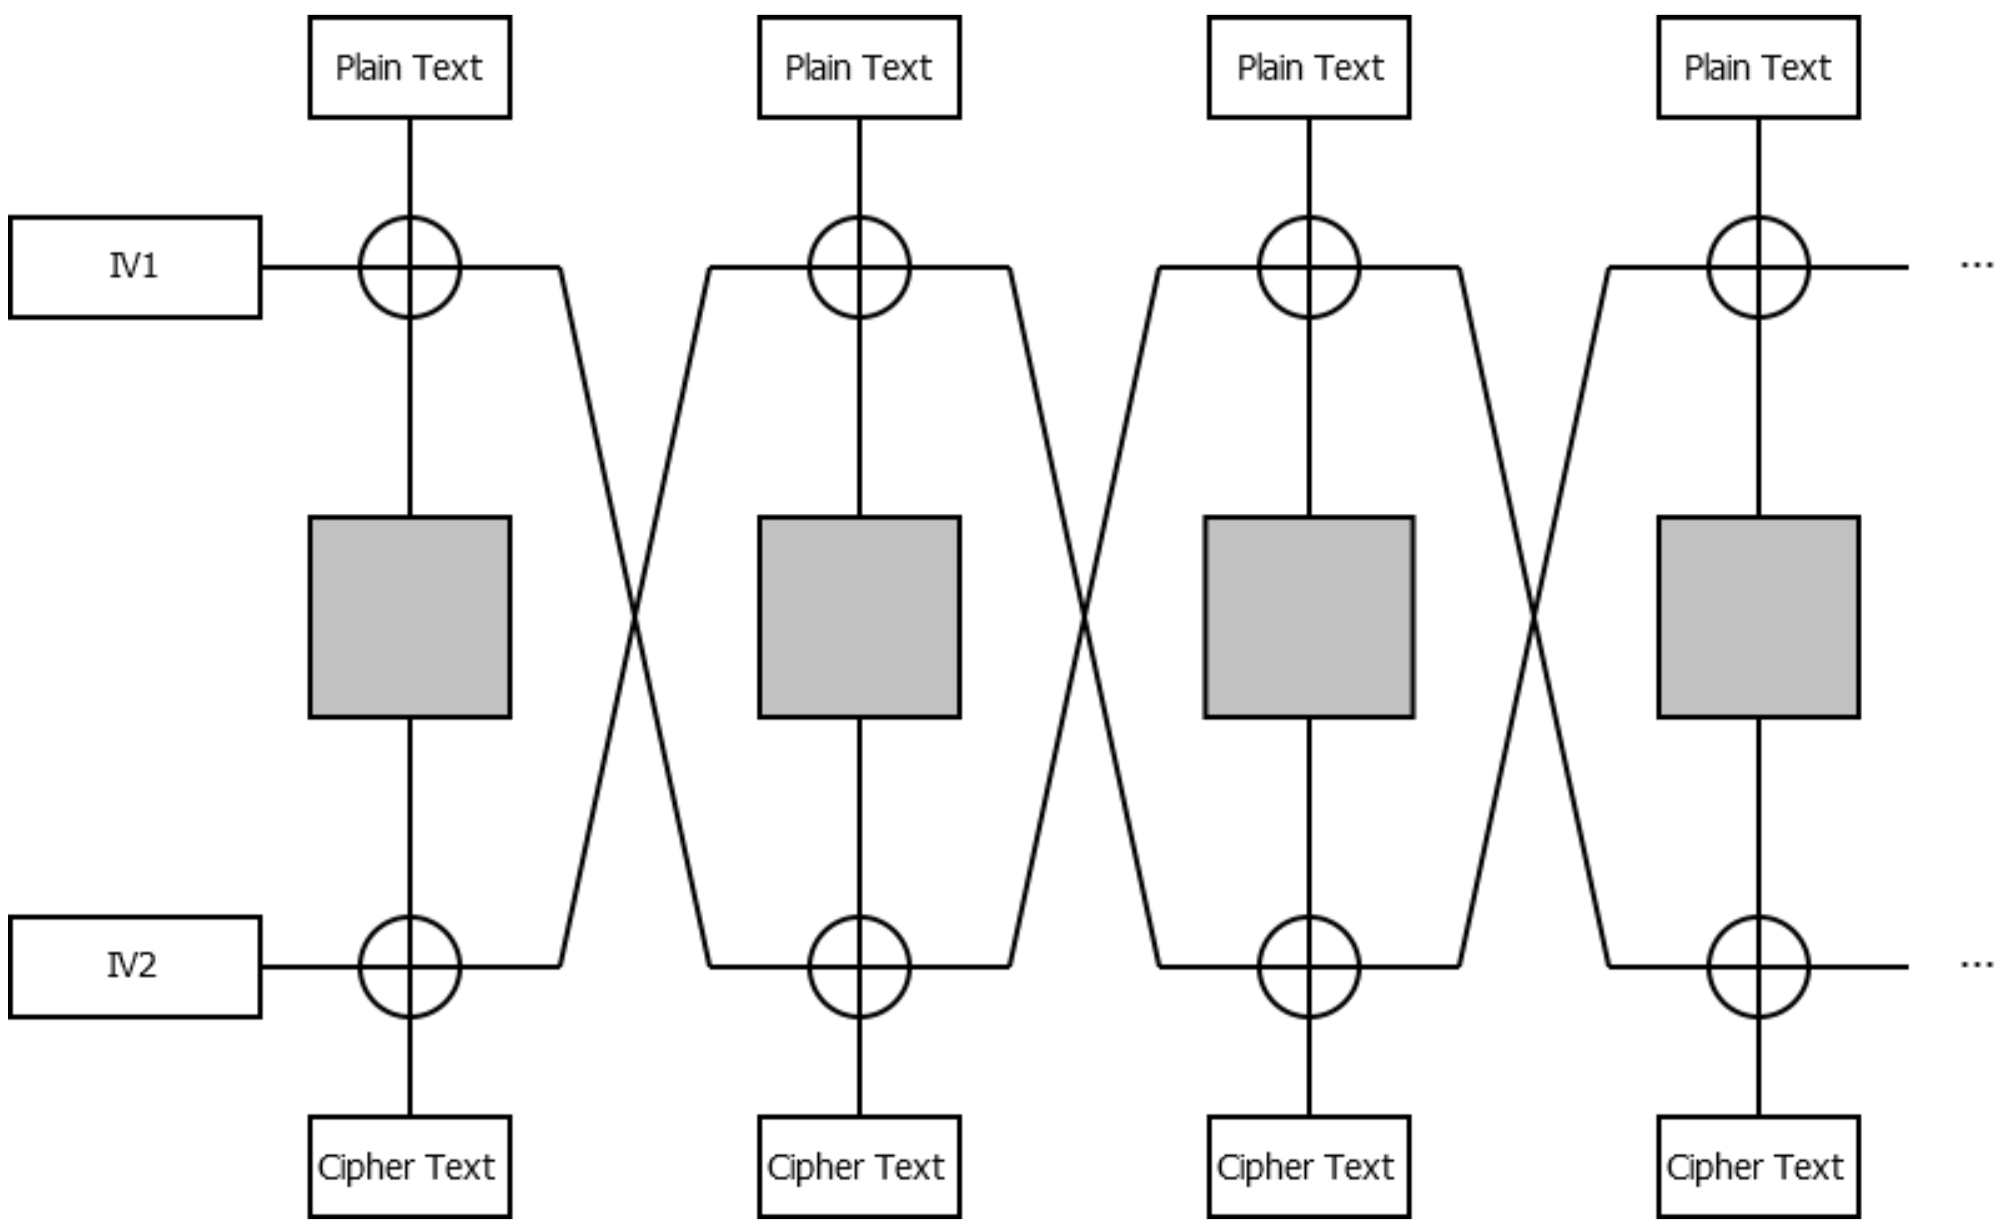
\includegraphics[width=3.5in]{xbc1.png}
\caption{The block diagram of XBC-1 operation.}
\label{fig_xbc1}
\end{figure}

\begin{algorithm}
 \caption{XBC-1}
 \label{alg-xbc1}
 \begin{algorithmic}
 \FOR{blocks $i=0$ to $n$}
 \STATE $IV_{i+1}^2 = PT_i \oplus IV_{i}^1$
 \STATE $i = BLOCKCIPHER(K, IV_{i+1}^2)$
 \STATE $CT_i = IV_{i+1}^1 = i \oplus IV_{i}^2$
 \ENDFOR
 \end{algorithmic}

 \noindent\rule{3.5in}{0.4pt}

 \begin{itemize}
   \item {$\mathbf{K}$}: The key for the underlying block cipher.
   \item {$\mathbf{IV_0^1}$}: The first provided initialization vector, must have length of the underlying block cipher.
   \item {$\mathbf{IV_0^2}$}: The second provided initialization vector, must have length of the underlying block cipher.
   \item {$\mathbf{PT}$}: The plain text, described as block $0$ to $n$.
   \item {$\mathbf{CT}$}: The cipher text blocks, described as block $0$ to $n$.
   \item {$\mathbf{IV_n^1}$}: The first initialization vector sent into round $n$.
   \item {$\mathbf{IV_n^2}$}: The second initialization vector sent into round $n$.
 \end{itemize}
\end{algorithm}

\subsection{Algorithm XBC-2}

The construction of this mode is a slight variant of XBC-1. See the figure \ref{fig_xbc2} and algorithm \ref{alg-xbc2}. The initial IV1 and IV2 are provided in the first round. The IV1 for each subsequent round of block cipher is obtained from the output of block cipher of the previous round. Similarly, the IV2 for each subsequent round of block cipher is obtained from the XOR of IV1 and the plaintext of the previous round similar to XBC-1.

\begin{figure}[!t]
\centering
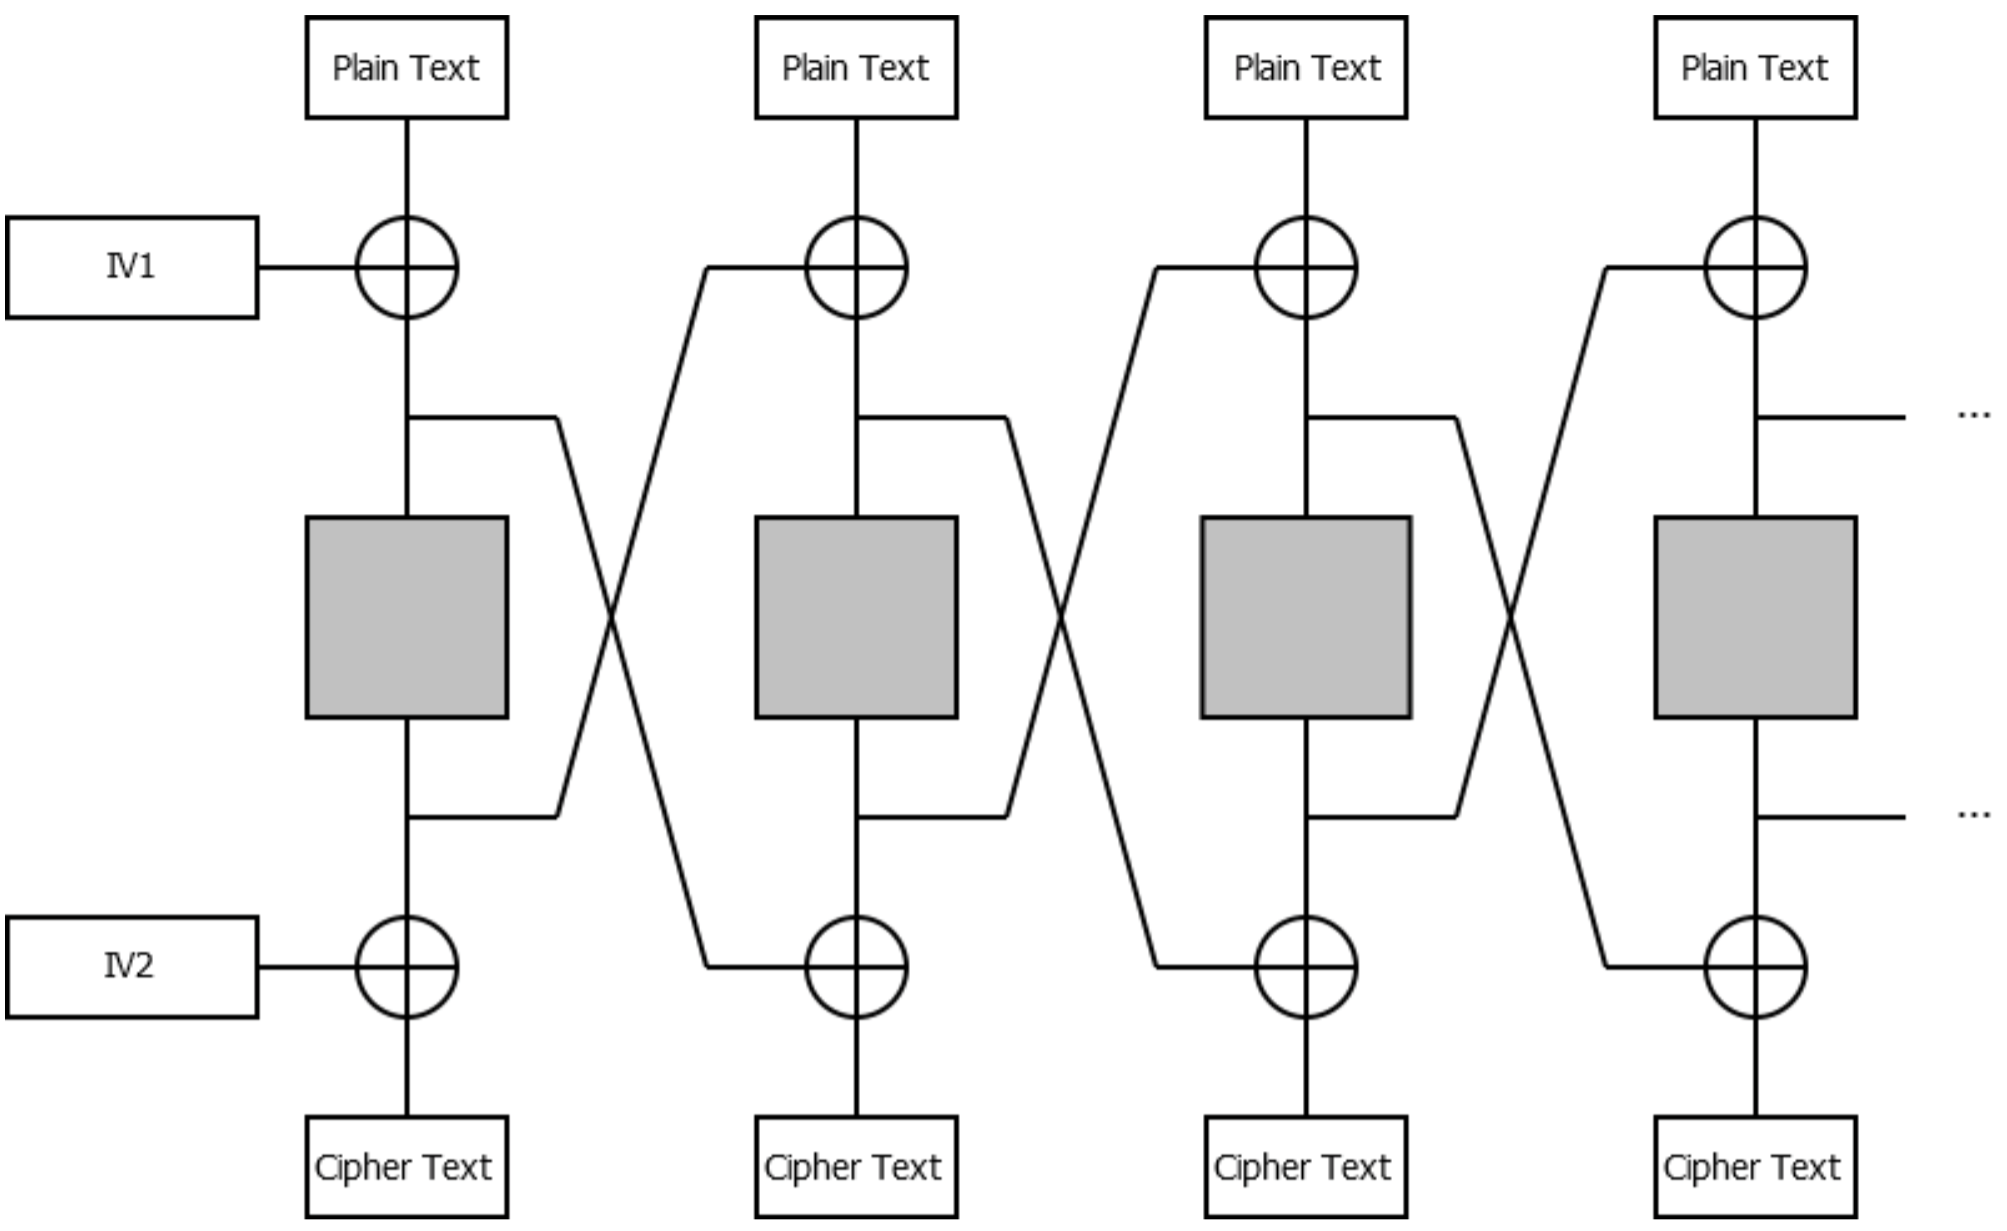
\includegraphics[width=3.5in]{xbc2.png}
\caption{The block diagram of XBC-2 operation.}
\label{fig_xbc2}
\end{figure}

\begin{algorithm}
 \caption{XBC-2}
 \label{alg-xbc2}
 \begin{algorithmic}
 \FOR{blocks $i=0$ to $n$}
 \STATE $IV_{i+1}^2 = PT_i \oplus IV_{i}^1$
 \STATE $i = BLOCKCIPHER(K, IV_{i+1}^2)$
 \STATE $CT_i = IV_{i+1}^1 \oplus IV_{i}^2$
 \ENDFOR
 \end{algorithmic}

 \noindent\rule{3.5in}{0.4pt}

 \begin{itemize}
   \item {$\mathbf{K}$}: The key for the underlying block cipher.
   \item {$\mathbf{IV_0^1}$}: The first provided initialization vector, must have length of the underlying block cipher.
   \item {$\mathbf{IV_0^2}$}: The second provided initialization vector, must have length of the underlying block cipher.
   \item {$\mathbf{PT}$}: The plain text, described as block $0$ to $n$.
   \item {$\mathbf{CT}$}: The cipher text blocks, described as block $0$ to $n$.
   \item {$\mathbf{IV_n^1}$}: The first initialization vector sent into round $n$.
   \item {$\mathbf{IV_n^2}$}: The second initialization vector sent into round $n$.
 \end{itemize}
\end{algorithm}

\section{Security analysis of different modes}

\subsection{IND-CCA security of both XBC modes}
One can break IND-CCA of both XBC-1 and XBC-2 with the same simple algorithm that works against schemes such as CBC\$. It is as follows:

For distinct n-bit strings $M_0$, $M_1$:

\begin{gather*}
  C \leftarrow LR_k (M_0, M_1) \\
  M \leftarrow D_k (C || 0^n) \\
  If\ M[0] == M_0\ return\ 0\ otherwise\ 1
\end{gather*}

The first block of M will be exactly what was encrypted by the encryption oracle, so we can simply compare that block with $M_0$ and $M_1$ and know which experiment we are in. The above attack will work every time.

\begin{gather*}
  Adv_{XBC-1}^{IND-CCA}(A) = 1 \\
  q_e=q_d=1,\ \mu_e = \mu_d = 2n \\
  t:\ compare,\ concat\ two\ n-bit\ strings \\
\end{gather*}

Assumed that theses schemes are IND-CPA secure, one can achieve IND-CCA security easily by using encrypt-then-MAC with some good MAC.

\subsection{INC-CPA security of XBC-1}

While the author doesn't state what the security of the scheme is  - we assume IND-CPA security - he mentions that for encryption of 1-2 blocks, XBC-1 can be used to create a two-man rule. He discusses a few situations where different parts of the secret key (which consists of the cipher key $k$, IV1, and IV2) are compromised by an adversary. Let us walk through these and other cases. \\

\subsubsection{Both IVs Compromised} \
\label{xbc1-both_IVs}

If an adversary acquires both the IV vectors, but not the cipher key $k$, we claim that the plaintext can still not be recovered since the blockcipher chosen will be a PRF, thus producing seemingly random output. However, the scheme is not IND-CPA secure under these circumstances, since we can let the messages be such that we can distinguish equality of the first blocks.

Let $i$ be the current index in the IV vectors. We can then look up the next IV1, IV2 in the vectors, and do the following attack:
\begin{gather*}
  C_0 \leftarrow LR_k(IV1_i, IV1_i) \\
  \Rightarrow C_0=E_k(IV1_i \oplus IV1_i) \oplus IV2_i \\
  = E_k(0^n) \oplus IV2_i \\
  C_1 \leftarrow LR_k(IV1_{i+1}, \overline{IV1_{i+1}}) \\ \\
  Let\ E_0=C_0 \oplus IV2_i=E_k(0^n) \\
  and\ E_1=C_1 \oplus IV2_{i+1}=E_k(0^n\ or\ 1^n) \\
  If\ E_0==E_1\ then\ return\ 0\ else\ 1
\end{gather*}
Note that the IVs should change each time, so by IV1 we mean whatever is in next in the vector, which is different when obtaining $C_1$ from when we obtained $C_0$. As such, the only information we can infer about the plaintexts from this lack of IND-CPA security is whether or not the plaintexts have the same relation to their respective IV1, i.e. whether
\begin{gather*}
  M_i[0] \oplus IV1_i == M_{i+1}[0] \oplus IV1_{i+1}
\end{gather*}

\subsubsection{Cipher key and one IV compromised} \
\label{xbc1-k_oneIV}

The paper discusses what happens if an adversary recovers one of the IVs and the cipher key $k$. This is interesting because in the situation of a two-man rule, we want it to be impossible for one of them to act without the other. The author states that if an adversary has IV1 and $k$, he cannot recover the plaintext, but an adversary given IV2 and $k$ can decrypt all but the first block. Consider the facts below which hold when one is given IV2 and $k$ for some ciphertext $C$ encrypted with XBC-1:

\begin{gather*}
  C[0] = E_k(M[0] \oplus IV1) \oplus IV2 \\
  C[1] = E_k(M[1] \oplus C[0]) \oplus (M[0] \oplus IV1) \\
  Can\ find\ X = E_k^{-1}(C[0] \oplus IV2) = M[0] \oplus IV1 \\
  \Rightarrow Know\ M[1] = E_k^{-1}(C[1] \oplus X) \oplus C[0]
\end{gather*}
In this situation, we know not only $M[1]$ but all that will be propagated to the next block, so we can decrypt that as well. In fact, we can decrypt all blocks but the first, since that block is essentially the One Time Pad given we don't know IV1.

The author suggests that because of this insecurity, we should not encrypt ``more than 1-2 blocks'' when using the two-man rule in this case, but we would advise to only encrypt one. Encrypting two blocks when one party knows IV2 and $k$ would mean that one member can recover half of every plaintext on his own!

In the case that we know IV1 and $k$
\begin{itemize}
 \item The output of the first block is XORed with IV2, which we do not know
 \item The second block will seem random to us, since $IV1 \oplus M[0]$, which is unknown, will propagate as IV2 for the second block.
 \item This pattern continues for all blocks, i.e. there will always be information unknown to us that propagates as an IV
\end{itemize}

However, if the plaintexts are predictable, i.e. we can identify plaintexts that have a high chance to be sent, we might be able to use the formula above for C[1] to gain information about the message. If we insert guesses for M[0] and M[1] into the formula, and use the values of $k$ and IV1 that we know, we can compare the result with C[1]. If they are equal, there is a good chance that the guesses are indeed the message blocks sent.

If our guess was correct, we know all the points that will propagate forward from the second block - the upper point being M[1] XOR C[0] - and can therefore decrypt all the following messages!

\subsubsection{One IV compromised} \

Since we do not know the other IV, the ciphertext will appear random to us just like output from the One Time Pad. Thus no information is leaked as long as we do not know the cipher key $k$. The scheme remains secure and the plaintexts uncompromised by any attacker with reasonable resources.

\subsubsection{Cipher key $k$ compromised} \

Since we do not know any of the IVs in this case, we have no clue what the input to nor output from the blockcipher was in the first block. Since unknown information propagates as IV2 to the following block, and unknown information will continue to propagate, the scheme remains secure.

\subsection{INC-CPA security of XBC-2}

Let us consider the security of XBC-2, which is assumed to be IND-CPA. The author suggests that this scheme can too be used to create a two-man rule. Let us again walk through the possible special cases that can occur if some information falls into the hands of an adversary, as is perhaps more likely when there are multiple parties keeping the secrets.

\subsubsection{Both IVs Compromised} \

Given both IV vectors but without the cipher key $k$, we again claim that an adversary cannot recover the plaintext, just like with XBC-1 \ref{xbc1-both_IVs}. Since the blockcipher is assumed to be a PRF, whatever comes out of it doesn't help us to decrypt the message. However, just as with XBC-1, we can tell from the output of the blockcipher if messages have the same relation to their respective IV1 in the sense that
\begin{gather*}
  M_i[0] \oplus IV1_i == M_{i+1}[0] \oplus IV1_{i+1}
\end{gather*}

We can exploit the above fact, and break IND-CPA security with the exact same adversary we used in \ref{xbc1-both_IVs}, since the output from the first block is the same for XBC-1 and XBC-2. Just as noted there, the only information this exploit gets us is whether or not the plaintexts have the same relation to their respective IV1, as explained in the previous paragraph.

\subsubsection{Cipher key and one IV compromised} \

A two-man rule is an interesting application of this scheme, and one would want to know the security implications if one party would be an adversary; what can he do without the other? \

Anyone with $k$ and IV2 can find what both the input and output of the first blockcipher was in the first block of the construction. We can't find $M[0]$ since it is XORed with IV1 which we don't know, but we still know all that will be propagated to the next block, and thus we can decrypt all but the first block, just as for XBC-1 (in \ref{xbc1-k_oneIV}). \

Given IV1 and k, we can't decrypt since IV2 is blocking us both from decrypting the first block and finding out what was propagated to the next block. This is the case because we don't know what IV2 is, nor what it was XORed with, so the output is just a random bitstring for us. In other words, it's impossible to decrypt the first block alone. \

However, the IND-CPA game is very easy to win: if we are the one providing the plaintext, i.e. we know the plaintext, IV1 and $k$, then we can decrypt all blocks but the first since IV2 is not propagated at all! An efficient example attack breaking IND-CPA is as below:
\begin{gather*}
  C \leftarrow LR_k(0^{2n},0^n || 1^n) \\
  Can't\ decrypt\ 1st\ block,\ however: \\
  C[1] = E_k(M[1] \oplus E_k(M[0] \oplus IV1) \oplus M[0] \oplus IV1) \\
  \Rightarrow E_k^{-1}(C[1] \oplus M[0] \oplus IV1) \\
  \oplus E_k(M[0] \oplus IV1) = M[1] \\
  Use\ M[1]\ from\ above,\ and\ run: \\
  If\ M[1]==0^n\ return\ 0\ otherwise\ 1
\end{gather*}

This would indicate that when an adversary is given the IV1 vector and $k$, security is weak if the plaintexts are predictable. If we have a limited number of guesses for the values of the first two blocks, we can verify whether or not $C[1]$ is possible with these values given what we know about $k$ and IV1. This means that an attacker given $k$, the IV1 vector and a ciphertext can have some sense of how likely it is that the ciphertext is the encryption some probable plaintext as compared to some other probable plaintext, which is very serious.

\subsubsection{One IV compromised} \
\label{xbc2-one_iv}

Given IV1, we can't tell anything from the ciphertext since the blockcipher is a PRF. Even in the IND-CPA game, where we decide (and thus know) the plaintexts, we can't tell anything since we can't decrypt with respect to the blockcipher, nor can we tell anything about the equality of messages assumed that IV2 changes between encryptions. However, if IV2 is fixed, i.e. reused every time, we can send messages in IND-CPA such that we can tell if the input to the blockcipher was equal, and thus break IND-CPA. But the scheme is IND-CPA in this case if IV2 changes, as it should. \

If we are given IV2, we can tell what the output from the block cipher was. That doesn't help us to decrypt the plaintext, and since we don't know $k$ we only know one of the two values propagating as IV for the following block. If IV1 is fixed, though, there is no randomness except IV2 which we know, and we can tell if two messages are equal since the output from the block cipher would then be equal too.

\subsubsection{Cipher key $k$ compromised} \

Without any knowledge of the IVs, we are helpless since we are essentially given the One Time Pad for each block of the output, which is Shannon secure. It would take for both IVs to be fixed for us to be able to tell anything, namely message equality. This is no surprise, since this and other previously mentioned cases where all IVs are either known or fixed have no unknown randomness in them.

\subsection{Conclusions of security in special cases}

The below table lists whether an adversary can decrypt parts or all of the plaintext given different parts of the secret key. \\

\begin{minipage}{6cm} % Footnotes don't work without using minipage
\begin{tabular}{| l | c c c c | }
\hline
  Scheme & Both IVs & One\ IV,\ k & One\ IV & k \\ \hline
  XBC-1 & N & Y\footnote{This holds only given k and IV2, but not for k and IV1.} & N & N \\
  XBC-2 & N & Y\footnote{This holds only given k and IV2. Given k and IV1, we may find information
  about the plaintexts if they are predictable.} & N & N \\
\hline
\end{tabular}
\end{minipage} \\

Below is the IND-CPA security in these cases. \\

\begin{tabular}{| l | c c c c | }
\hline
  Scheme & Both IVs & One\ IV,\ k & One\ IV & k \\ \hline
  XBC-1 & N & N & Y & Y \\
  XBC-2 & N & N & Y & Y \\
\hline
\end{tabular} \\

Some general takeaways from considering these cases is that

\begin{enumerate}
  \item If you reuse IVs, you risk ruining randomness and making the scheme deterministic, thus leaking message equality and ruining IND-CPA. This is especially true in the case where an adversary acquires inside information in the form of an IV.
  \item Never let one party possess both $k$ and IV2
  \item No situation where one person possesses two of the three secrets is ideal, so the schemes are only secure if encrypting one block, which is impractical and therefore these schemes are not good for creating a two-man rule
  \item Security of possible distributions of the three secrets among two persons will be analyzed under the Implementation Guidelines section
\end{enumerate}

\section{Implementation guidelines}

% {\color{red}
% TODO: Let’s write about how the scheme should be used practically!
% \begin{itemize}
%   \item How should we use IV vectors? (remember to consider generators vs occasionally agreeing on new vectors using this very scheme)
%   \item Do we need to change both every time?
%   \item Can we use the same k all the time?
% \end{itemize}
% We can motivate these things with references to the security analysis!
% }

Let us consider what one should be aware of when using this scheme in practice. One problem with this scheme is that we need a new IV1 and IV2 for each round. If we imagine using hybrid encryption to synchronize the blockcipher key and initial IV vectors. When we start running out of IVs, we can encrypt new vectors and send them using this very encryption scheme. Note that whatever the number of blocks in the message, we just need one of each IV to encrypt it. Thus we can encrypt very large vectors of new IVs. However, we'd rather not have to send large things over the network if we can avoid it. A more elegant solution would be to use PRGs, or Pseudo-Random Generators. In that case, we'd use the assymetric part of the hybrid encryption scheme to agree on the key of the blockcipher key and an initial seed for each generator, which is to be used with the PRGs.

But do we need to change both IVs every time? Well, we saw in \ref{xbc2-one_iv} that randomness is necessary to achieve the highest security this scheme can offer. It is therefore strongly advised to always use good random IVs.

However, in these experiments I have assumed that we keep using the same blockcipher key forever, and the security is still good. Therefore one does not need to worry about changing it.

% conference papers do not normally have an appendix


% use section* for acknowledgement
\section*{Acknowledgment}

We would like to show our gratitude to Dr. Alexandra Boldyreva, Georgia Tech for sharing her pearls of wisdom with us during the Applied Cryptography course and her guidance received while working on this project.






% trigger a \newpage just before the given reference
% number - used to balance the columns on the last page
% adjust value as needed - may need to be readjusted if
% the document is modified later
%\IEEEtriggeratref{8}
% The "triggered" command can be changed if desired:
%\IEEEtriggercmd{\enlargethispage{-5in}}

% references section

% can use a bibliography generated by BibTeX as a .bbl file
% BibTeX documentation can be easily obtained at:
% http://www.ctan.org/tex-archive/biblio/bibtex/contrib/doc/
% The IEEEtran BibTeX style support page is at:
% http://www.michaelshell.org/tex/ieeetran/bibtex/
%\bibliographystyle{IEEEtran}
% argument is your BibTeX string definitions and bibliography database(s)
%\bibliography{IEEEabrv,../bib/paper}
%
% <OR> manually copy in the resultant .bbl file
% set second argument of \begin to the number of references
% (used to reserve space for the reference number labels box)
\begin{thebibliography}{1}

\bibitem{watson}
Andre Watson, \emph{Cross Block Chaining (XBC)}.\hskip 1em plus
  0.5em minus 0.4em\relax May, 2014.

\end{thebibliography}

% that's all folks
\end{document}


